\documentclass[border=3pt]{standalone}
\usepackage{fontspec}
\setmainfont{Times New Roman}
\usepackage{pgfplots}
\pgfplotsset{compat=1.18}
\usetikzlibrary{arrows.meta,calc,positioning,shapes.geometric}
\definecolor{forest}{HTML}{346E57}
\definecolor{sage}{HTML}{E8EFEA}
\definecolor{clay}{HTML}{B77E60}
\definecolor{gray}{HTML}{718078}
\definecolor{rule}{HTML}{B7C3BA}
\definecolor{ink}{HTML}{000000}
\begin{document}
\hyphenpenalty=10000\exhyphenpenalty=10000
\fontsize{10}{12}\selectfont
\renewcommand{\small}{\fontsize{9}{11}\selectfont}
\renewcommand{\scriptsize}{\fontsize{8}{10}\selectfont}
\resizebox{16cm}{!}{%
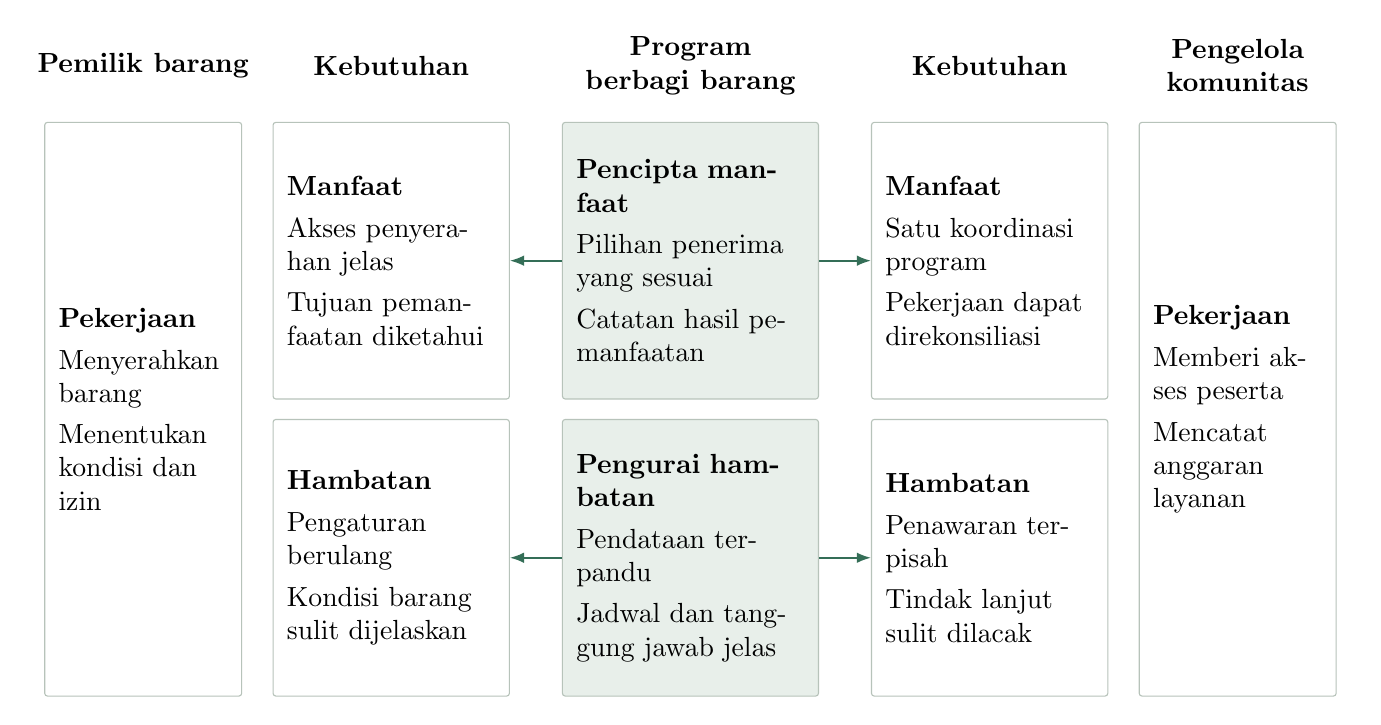
\begin{tikzpicture}[x=1cm,y=1cm,box/.style={draw=rule,fill=white,rounded corners=1pt,align=left,inner sep=5pt},head/.style={align=center,font=\bfseries}]
\node[head,text width=2.7cm]at(0,4.362962962962962){Pemilik barang};
\node[head,text width=2.7cm]at(3.15,4.362962962962962){Kebutuhan};
\node[head,text width=2.7cm]at(6.95,4.362962962962962){Program berbagi barang};
\node[head,text width=2.7cm]at(10.75,4.362962962962962){Kebutuhan};
\node[head,text width=2.7cm]at(13.9,4.362962962962962){Pengelola komunitas};
\node[box,text width=2.15cm,minimum height=7.285925925925925cm] at(0,0){\textbf{Pekerjaan}\par\smallskip Menyerahkan barang\par\smallskip Menentukan kondisi dan izin};
\node[box,text width=2.15cm,minimum height=7.285925925925925cm] at(13.9,0){\textbf{Pekerjaan}\par\smallskip Memberi akses peserta\par\smallskip Mencatat anggaran layanan};
\node[box,text width=2.65cm,minimum height=3.5129629629629626cm] (leftgains) at(3.15,1.8864814814814812){\textbf{Manfaat}\par\smallskip Akses penyerahan jelas\par\smallskip Tujuan pemanfaatan diketahui};
\node[box,text width=2.65cm,minimum height=3.5129629629629626cm] (leftpains) at(3.15,-1.8864814814814812){\textbf{Hambatan}\par\smallskip Pengaturan berulang\par\smallskip Kondisi barang sulit dijelaskan};
\node[box,text width=2.65cm,minimum height=3.5129629629629626cm] (rightgains) at(10.75,1.8864814814814812){\textbf{Manfaat}\par\smallskip Satu koordinasi program\par\smallskip Pekerjaan dapat direkonsiliasi};
\node[box,text width=2.65cm,minimum height=3.5129629629629626cm] (rightpains) at(10.75,-1.8864814814814812){\textbf{Hambatan}\par\smallskip Penawaran terpisah\par\smallskip Tindak lanjut sulit dilacak};
\node[box,fill=sage,text width=2.9cm,minimum height=3.5129629629629626cm] (gain_creators)at(6.95,1.8864814814814812){\textbf{Pencipta manfaat}\par\smallskip Pilihan penerima yang sesuai\par\smallskip Catatan hasil pemanfaatan};
\node[box,fill=sage,text width=2.9cm,minimum height=3.5129629629629626cm] (pain_relievers)at(6.95,-1.8864814814814812){\textbf{Pengurai hambatan}\par\smallskip Pendataan terpandu\par\smallskip Jadwal dan tanggung jawab jelas};
\draw[-{Latex[length=1.8mm]},forest,line width=.6pt](gain_creators.west)--(leftgains.east);
\draw[-{Latex[length=1.8mm]},forest,line width=.6pt](gain_creators.east)--(rightgains.west);
\draw[-{Latex[length=1.8mm]},forest,line width=.6pt](pain_relievers.west)--(leftpains.east);
\draw[-{Latex[length=1.8mm]},forest,line width=.6pt](pain_relievers.east)--(rightpains.west);
\end{tikzpicture}
}

\end{document}
